\documentclass[12pt]{article}
\usepackage[english]{babel}
\usepackage{natbib}
\usepackage{url}
\usepackage[utf8x]{inputenc}
\usepackage{amsmath}
\usepackage{graphicx}
\graphicspath{{images/}}
\usepackage{parskip}
\usepackage{fancyhdr}
\usepackage{vmargin}
\usepackage{xcolor}
\usepackage{siunitx}
\usepackage{physics}
\setmarginsrb{3 cm}{2 cm}{3 cm}{2 cm}{1 cm}{1.5 cm}{1 cm}{1.5 cm}

\title{Lab 04}													% Title
\author{G 03}														% Author
\date{2 Apr 2019}														% Date

\makeatletter
\let\thetitle\@title
\let\theauthor\@author
\let\thedate\@date
\makeatother

\pagestyle{fancy}
\fancyhf{}
\rhead{\theauthor}
\lhead{\thetitle}
\cfoot{\thepage}
\newcommand{\mis}[3]{(#1 \pm #2) \ #3}
\newcommand{\misp}[3]{(#1 \#3 \pm #2}
\begin{document}

%%%%%%%%%%%%%%%%%%%%%%%%%%%%%%%%%%%%%%%%%%%%%%%%%%%%%%%%%%%%%%%%%%%%%%%%%%%%%%%%%%%%%%%%%

\begin{titlepage}
	\centering
    \vspace*{0.5 cm}
    
\includegraphics[scale = 0.75]{polito.jpg}\\[1.0 cm]				% University Logo
    \textsc{\LARGE Politecnico di Torino}\\[2.0 cm]						% University Name
	\textsc{\Large Digital systems electronics\\ A.A. 2018/2019}\\[0.5 cm]		% Course Code
	\textsc{\Large Prof. G. Masera}\\[0.5 cm]		% Nome del Professore
	\rule{\linewidth}{0.2 mm} \\[0.4 cm]
	{ \huge \bfseries \thetitle \\ \small \thedate}\\
	\rule{\linewidth}{0.2 mm} \\[1.5 cm]
	
	\begin{minipage}{0.4\textwidth}
		\begin{flushleft} \large
			Berchialla Luca\\												%Cognomi e nomi
			Laurasi Gjergji
			\\
			
			Mattei Andrea\\
            Lombardo Domenico Maria\\
            
			\end{flushleft}
			\end{minipage}~
			\begin{minipage}{0.4\textwidth}
            
			\begin{flushright} \large
			236032\\													%Matricole
			238259\\
            233755\\
            233959\\
            
		\end{flushright}
        
	\end{minipage}\\[2 cm]
	
\end{titlepage}

%%%%%%%%%%%%%%%%%%%%%%%%%%%%%%%%%%%%%%%%%%%%%%%%%%%%%%%%%%%%%%%%%%%%%%%%%%%%%%%%%%%%%%%%%
\newpage

\section{Gated SR latch}

The circuit shown in $figure\;1$ implements a gated SR latch.
Once coded into VHDL the Quartus Prime compiler uses separate memory components as shown in $figure\;2$ to depict the electric circuit.

\begin{figure}[h]
	\centering
    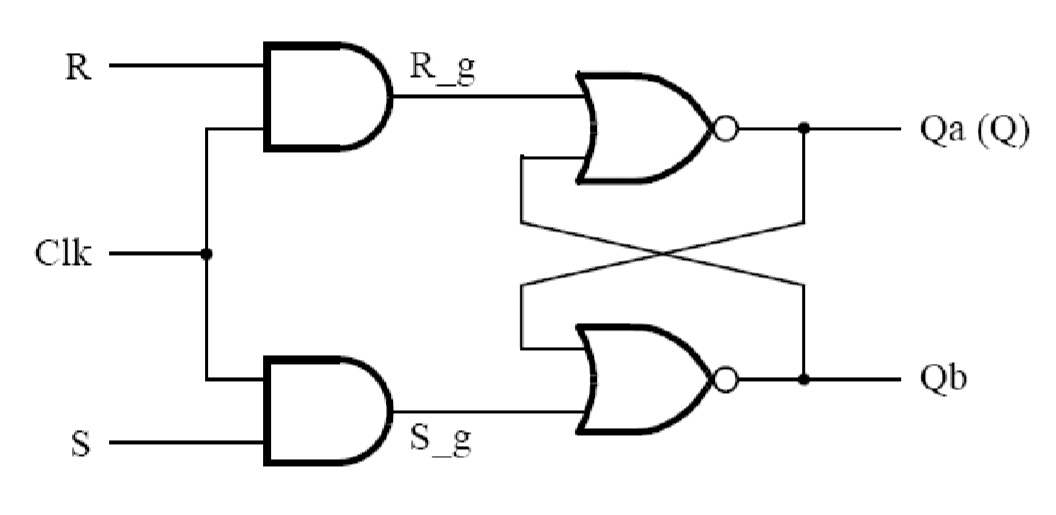
\includegraphics[scale = 0.75]{immagini/SRff.PNG}
    \caption{A gated SR latch circuit}		
\end{figure}

\begin{figure}[h]
	\centering
	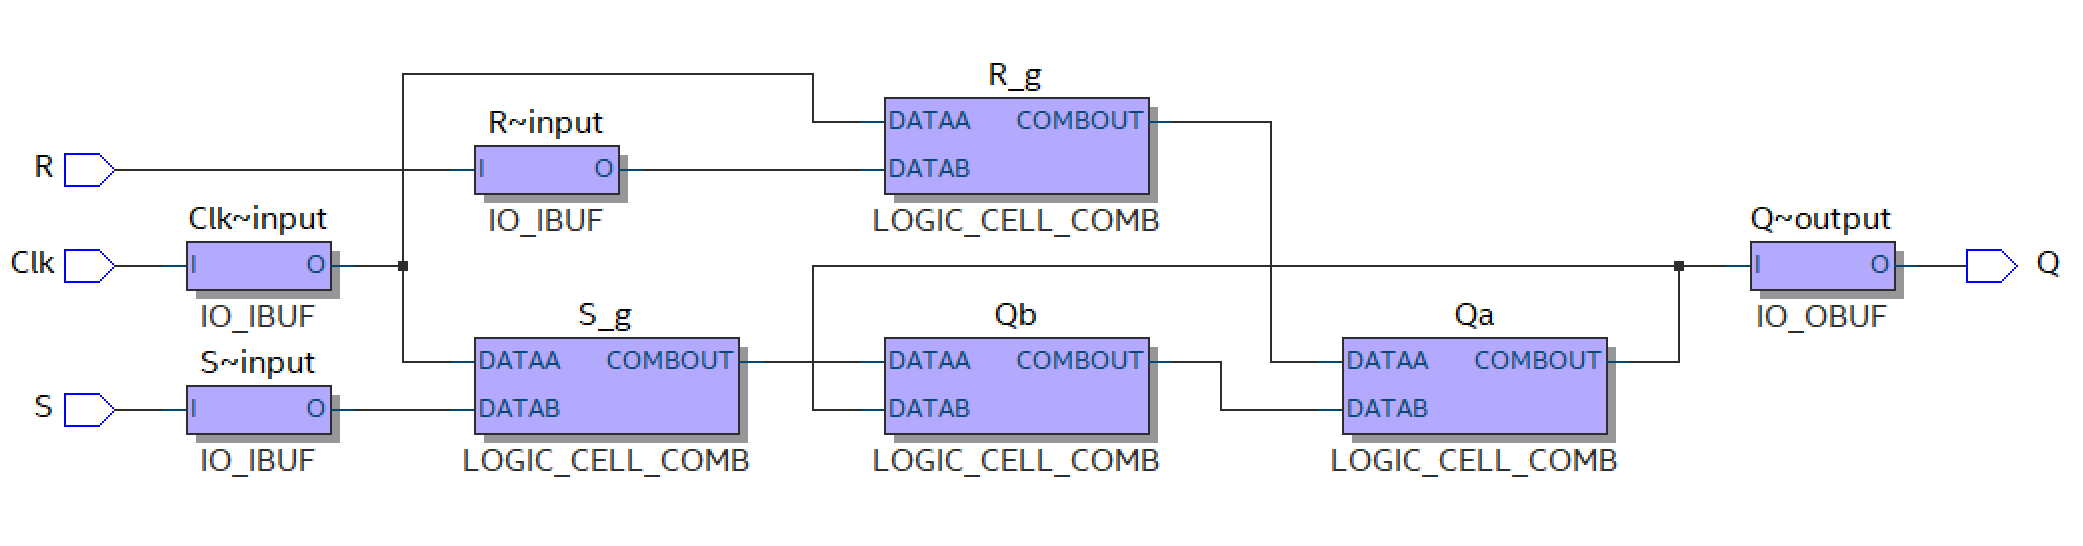
\includegraphics[scale = 0.6]{immagini/postmap.PNG}
	\caption{Quartus circuit implementation}
\end{figure}
\vspace{5mm}
Finally, a testbench has been written to test the behavior of the circuit, according to the table shown below:
\vspace{5mm}
\begin{figure}[h]
	\centering
	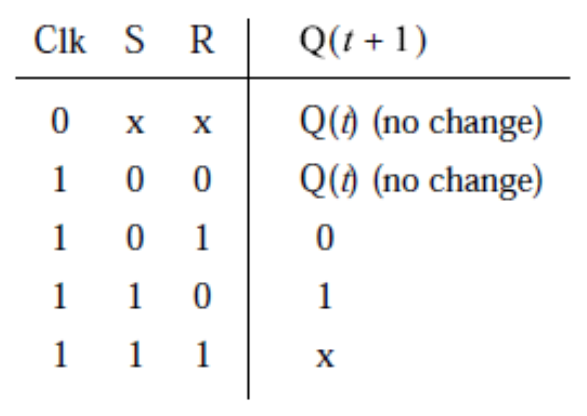
\includegraphics[scale = 0.6]{immagini/table_sr.PNG}		
\end{figure}
\newpage


\begin{figure}[h]
	\centering
	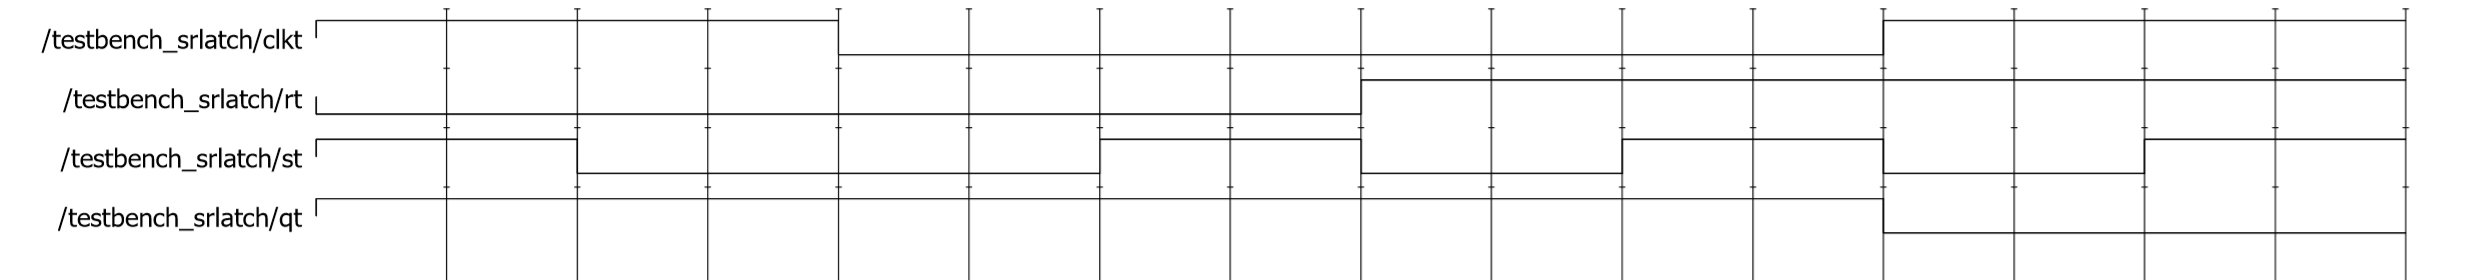
\includegraphics[scale = 0.45]{immagini/testbench1.PNG}
	\caption{Modelsim Testbench waves}
\end{figure}
The testbench results are shown by means of the simulated waves shown in $figure\;3$. 
Initially $CLK=1$, the lath is enabled. For $S=1$, $R=0$ the set condition is triggered and $Q=1$. Viceversa $Q=0$ when $S=0$, $R=1$, in reset condition. Once $CLK=0$ the latch is disabled entering in the memory condition as $S=0$, $R=0$. In the other hand for $S=1$, $R=1$ the latch behavior becomes unpredictable.
\vspace{10mm}
\section{16-bit synchronous counter}

The circuit in $figure\;4$ implements a 4-bit counter using T flip flops. A 16-bit version has been implemented using the same structure. Using the Quartus tools the maximum working frequency has been identified to be equal to $F=374.53MHz$ as reported in $figure\;5$ using a total of $31$ LEs.



\vspace{10mm}
\begin{figure}[h]
	\centering
	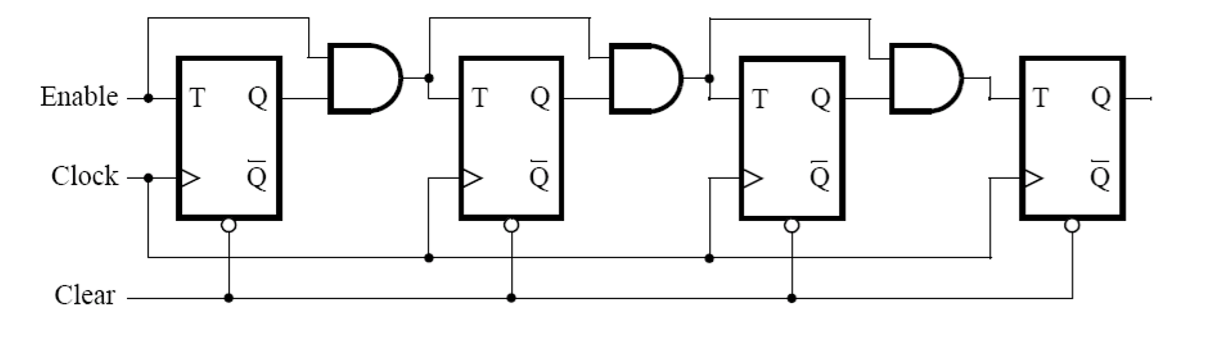
\includegraphics[scale = 0.8]{immagini/count.PNG}
	\caption{4-bit counter}
\end{figure}
\vspace{10mm}
	\begin{figure}[h]
		\centering
		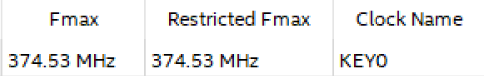
\includegraphics[scale = 0.9]{immagini/fmax.PNG}
		\caption{Maximum working frequency}
	\end{figure}
\newpage
Finally a testbench had been designed to check the functionality of the circuit, the results are shown in $figure\;6$ where the counting process is shown using the HEX display. Notice that the circuit is firstly initialized resetting the current state of every FF. Then the counting process has been started enabling the circuit and applying a clock to every FF.
		\begin{figure}[h]
			\centering
			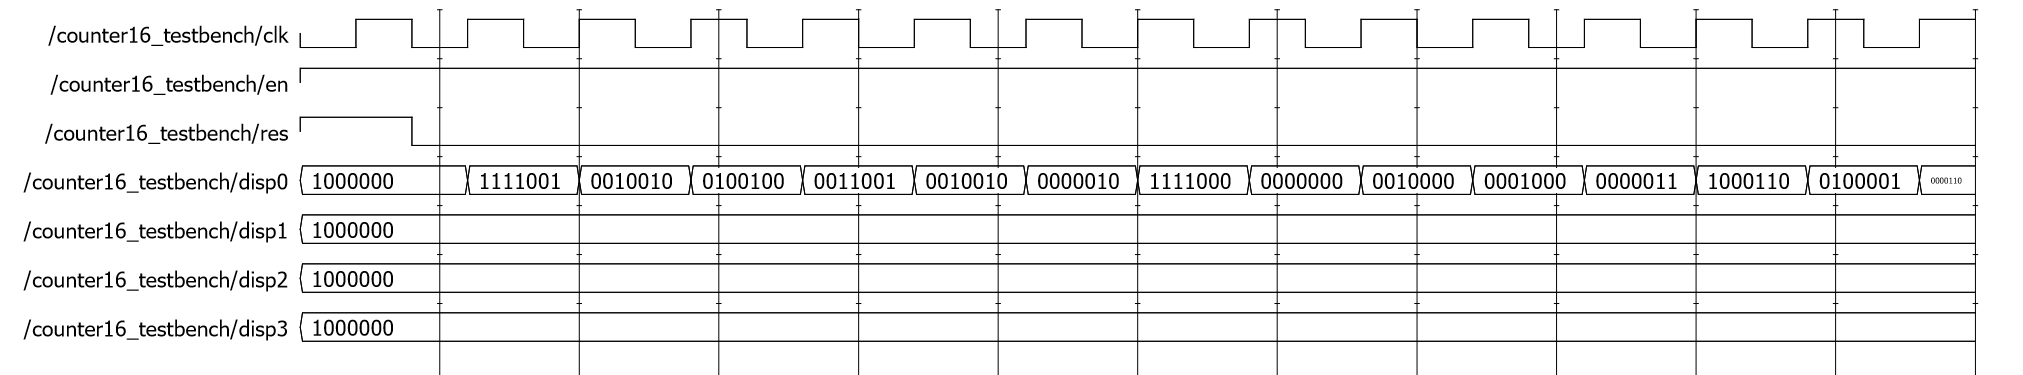
\includegraphics[scale = 0.6]{immagini/testbench2.PNG}
			\caption{Modelsim Testbench waves}
\end{figure}


\end{document}
